\section{Bayesian Inference on Constrained Stochastic Samples}
\label{sec:bayesian-inference}

This section presents the mathematical foundations for Bayesian inference on samples collected through constrained stochastic sampling with fuzzy window constraints. The Bayesian inference engine constitutes the Moon Landing Algorithm's third analytical layer, transforming sample collections into probabilistic understanding structures through rigorous posterior analysis.

\subsection{Mathematical Framework for Posterior Inference}

\begin{definition}[Bayesian Inference on Constrained Samples]
Let $\mathcal{D} = \{(x_i, w_i)\}_{i=1}^N$ represent a collection of constrained stochastic samples where $x_i \in \mathbb{R}^d$ denotes sample positions and $w_i \in [0,1]$ represents fuzzy window weights. The Bayesian inference process estimates posterior distributions $p(\theta|\mathcal{D})$ over parameter space $\Theta$.
\end{definition}

The likelihood function for constrained samples follows a weighted mixture model:

\begin{equation}
p(\mathcal{D}|\theta) = \prod_{i=1}^N \left[ \sum_{k=1}^K \pi_k \mathcal{N}(x_i; \mu_k, \Sigma_k) \right]^{w_i}
\label{eq:constrained-likelihood}
\end{equation}

where $\theta = \{\pi_k, \mu_k, \Sigma_k\}_{k=1}^K$ represents mixture parameters with $\pi_k$ denoting mixture weights, $\mu_k \in \mathbb{R}^d$ component means, and $\Sigma_k \in \mathbb{R}^{d \times d}$ positive definite covariance matrices.

\subsection{Prior Specifications and Hierarchical Modeling}

The hierarchical prior structure ensures proper Bayesian inference:

\begin{align}
\mu_k &\sim \mathcal{N}(\mu_0, \Lambda_0^{-1}) \label{eq:mean-prior}\\
\Sigma_k^{-1} &\sim \mathcal{W}(\nu_0, S_0) \label{eq:precision-prior}\\
\pi &\sim \text{Dir}(\alpha_1, \ldots, \alpha_K) \label{eq:mixture-prior}
\end{align}

where $\mathcal{W}(\nu_0, S_0)$ denotes the Wishart distribution with degrees of freedom $\nu_0$ and scale matrix $S_0$, and $\text{Dir}(\alpha_1, \ldots, \alpha_K)$ represents the Dirichlet distribution with concentration parameters $\alpha_k$.

\subsection{Posterior Sampling via Variational Bayes}

The posterior distribution $p(\theta|\mathcal{D})$ is approximated using variational Bayesian Gaussian mixture models. The variational lower bound maximization leads to the update equations:

\begin{align}
\text{E-step: } \gamma_{ik} &= \frac{\pi_k \mathcal{N}(x_i; \mu_k, \Sigma_k)^{w_i}}{\sum_{j=1}^K \pi_j \mathcal{N}(x_i; \mu_j, \Sigma_j)^{w_i}} \label{eq:responsibility}\\
\text{M-step: } \pi_k &= \frac{1}{N} \sum_{i=1}^N \gamma_{ik} \label{eq:mixture-update}\\
\mu_k &= \frac{\sum_{i=1}^N \gamma_{ik} w_i x_i}{\sum_{i=1}^N \gamma_{ik} w_i} \label{eq:mean-update}\\
\Sigma_k &= \frac{\sum_{i=1}^N \gamma_{ik} w_i (x_i - \mu_k)(x_i - \mu_k)^T}{\sum_{i=1}^N \gamma_{ik} w_i} + \lambda I_d \label{eq:covariance-update}
\end{align}

where $\gamma_{ik}$ represents the responsibility of component $k$ for sample $i$, and $\lambda > 0$ ensures positive definiteness.

\subsection{Understanding Extraction and Semantic Clustering}

\begin{definition}[Semantic Cluster Extraction]
From posterior samples $\{\theta^{(s)}\}_{s=1}^S$, semantic clusters $\mathcal{C} = \{C_k\}_{k=1}^K$ are extracted where each cluster $C_k$ is characterized by:
\begin{align}
C_k = \{&\text{center}: \bar{\mu}_k, \text{uncertainty}: \sigma_k, \\
&\text{importance}: \bar{\pi}_k, \text{volume}: \det(\bar{\Sigma}_k)^{1/2}\}
\end{align}
\end{definition}

The uncertainty quantification employs posterior variance estimation:

\begin{equation}
\sigma_k^2 = \frac{1}{S-1} \sum_{s=1}^S (\mu_k^{(s)} - \bar{\mu}_k)(\mu_k^{(s)} - \bar{\mu}_k)^T
\label{eq:posterior-variance}
\end{equation}

\subsection{Convergence Diagnostics and Quality Assessment}

The effective sample size (ESS) provides convergence assessment:

\begin{equation}
\text{ESS} = \frac{S^2}{\sum_{s=1}^S \exp(2(L^{(s)} - L_{\max}))}
\label{eq:effective-sample-size}
\end{equation}

where $L^{(s)}$ denotes the log-likelihood of sample $s$ and $L_{\max} = \max_s L^{(s)}$.

\begin{definition}[Cluster Separation Metric]
The Mahalanobis-based cluster separation quantifies semantic distinctness:
\begin{equation}
\text{Sep}(C_i, C_j) = \sqrt{(\mu_i - \mu_j)^T \left(\frac{\Sigma_i + \Sigma_j}{2}\right)^{-1} (\mu_i - \mu_j)}
\label{eq:cluster-separation}
\end{equation}
\end{definition}

\subsection{Confidence Interval Construction}

Credible intervals for cluster parameters follow from posterior samples:

\begin{equation}
\text{CI}_{1-\alpha}(\mu_k) = \left[ \bar{\mu}_k \pm z_{1-\alpha/2} \sqrt{\text{diag}(\sigma_k^2)} \right]
\label{eq:credible-intervals}
\end{equation}

where $z_{1-\alpha/2}$ represents the $(1-\alpha/2)$ quantile of the standard normal distribution.

\subsection{Computational Complexity and Scalability}

The computational complexity of the variational Bayesian inference scales as $\mathcal{O}(NdK + d^3K)$ per iteration, where $N$ represents sample count, $d$ dimensional complexity, and $K$ mixture components. The weighted likelihood evaluation introduces an additional factor proportional to the effective sample size $N_{\text{eff}} = \sum_{i=1}^N w_i$.

This Bayesian inference framework enables robust extraction of probabilistic understanding from constrained stochastic samples, providing the foundational mechanism for semantic interpretation within the Moon Landing Algorithm's hierarchical processing architecture.

\begin{figure}[htbp]
\centering
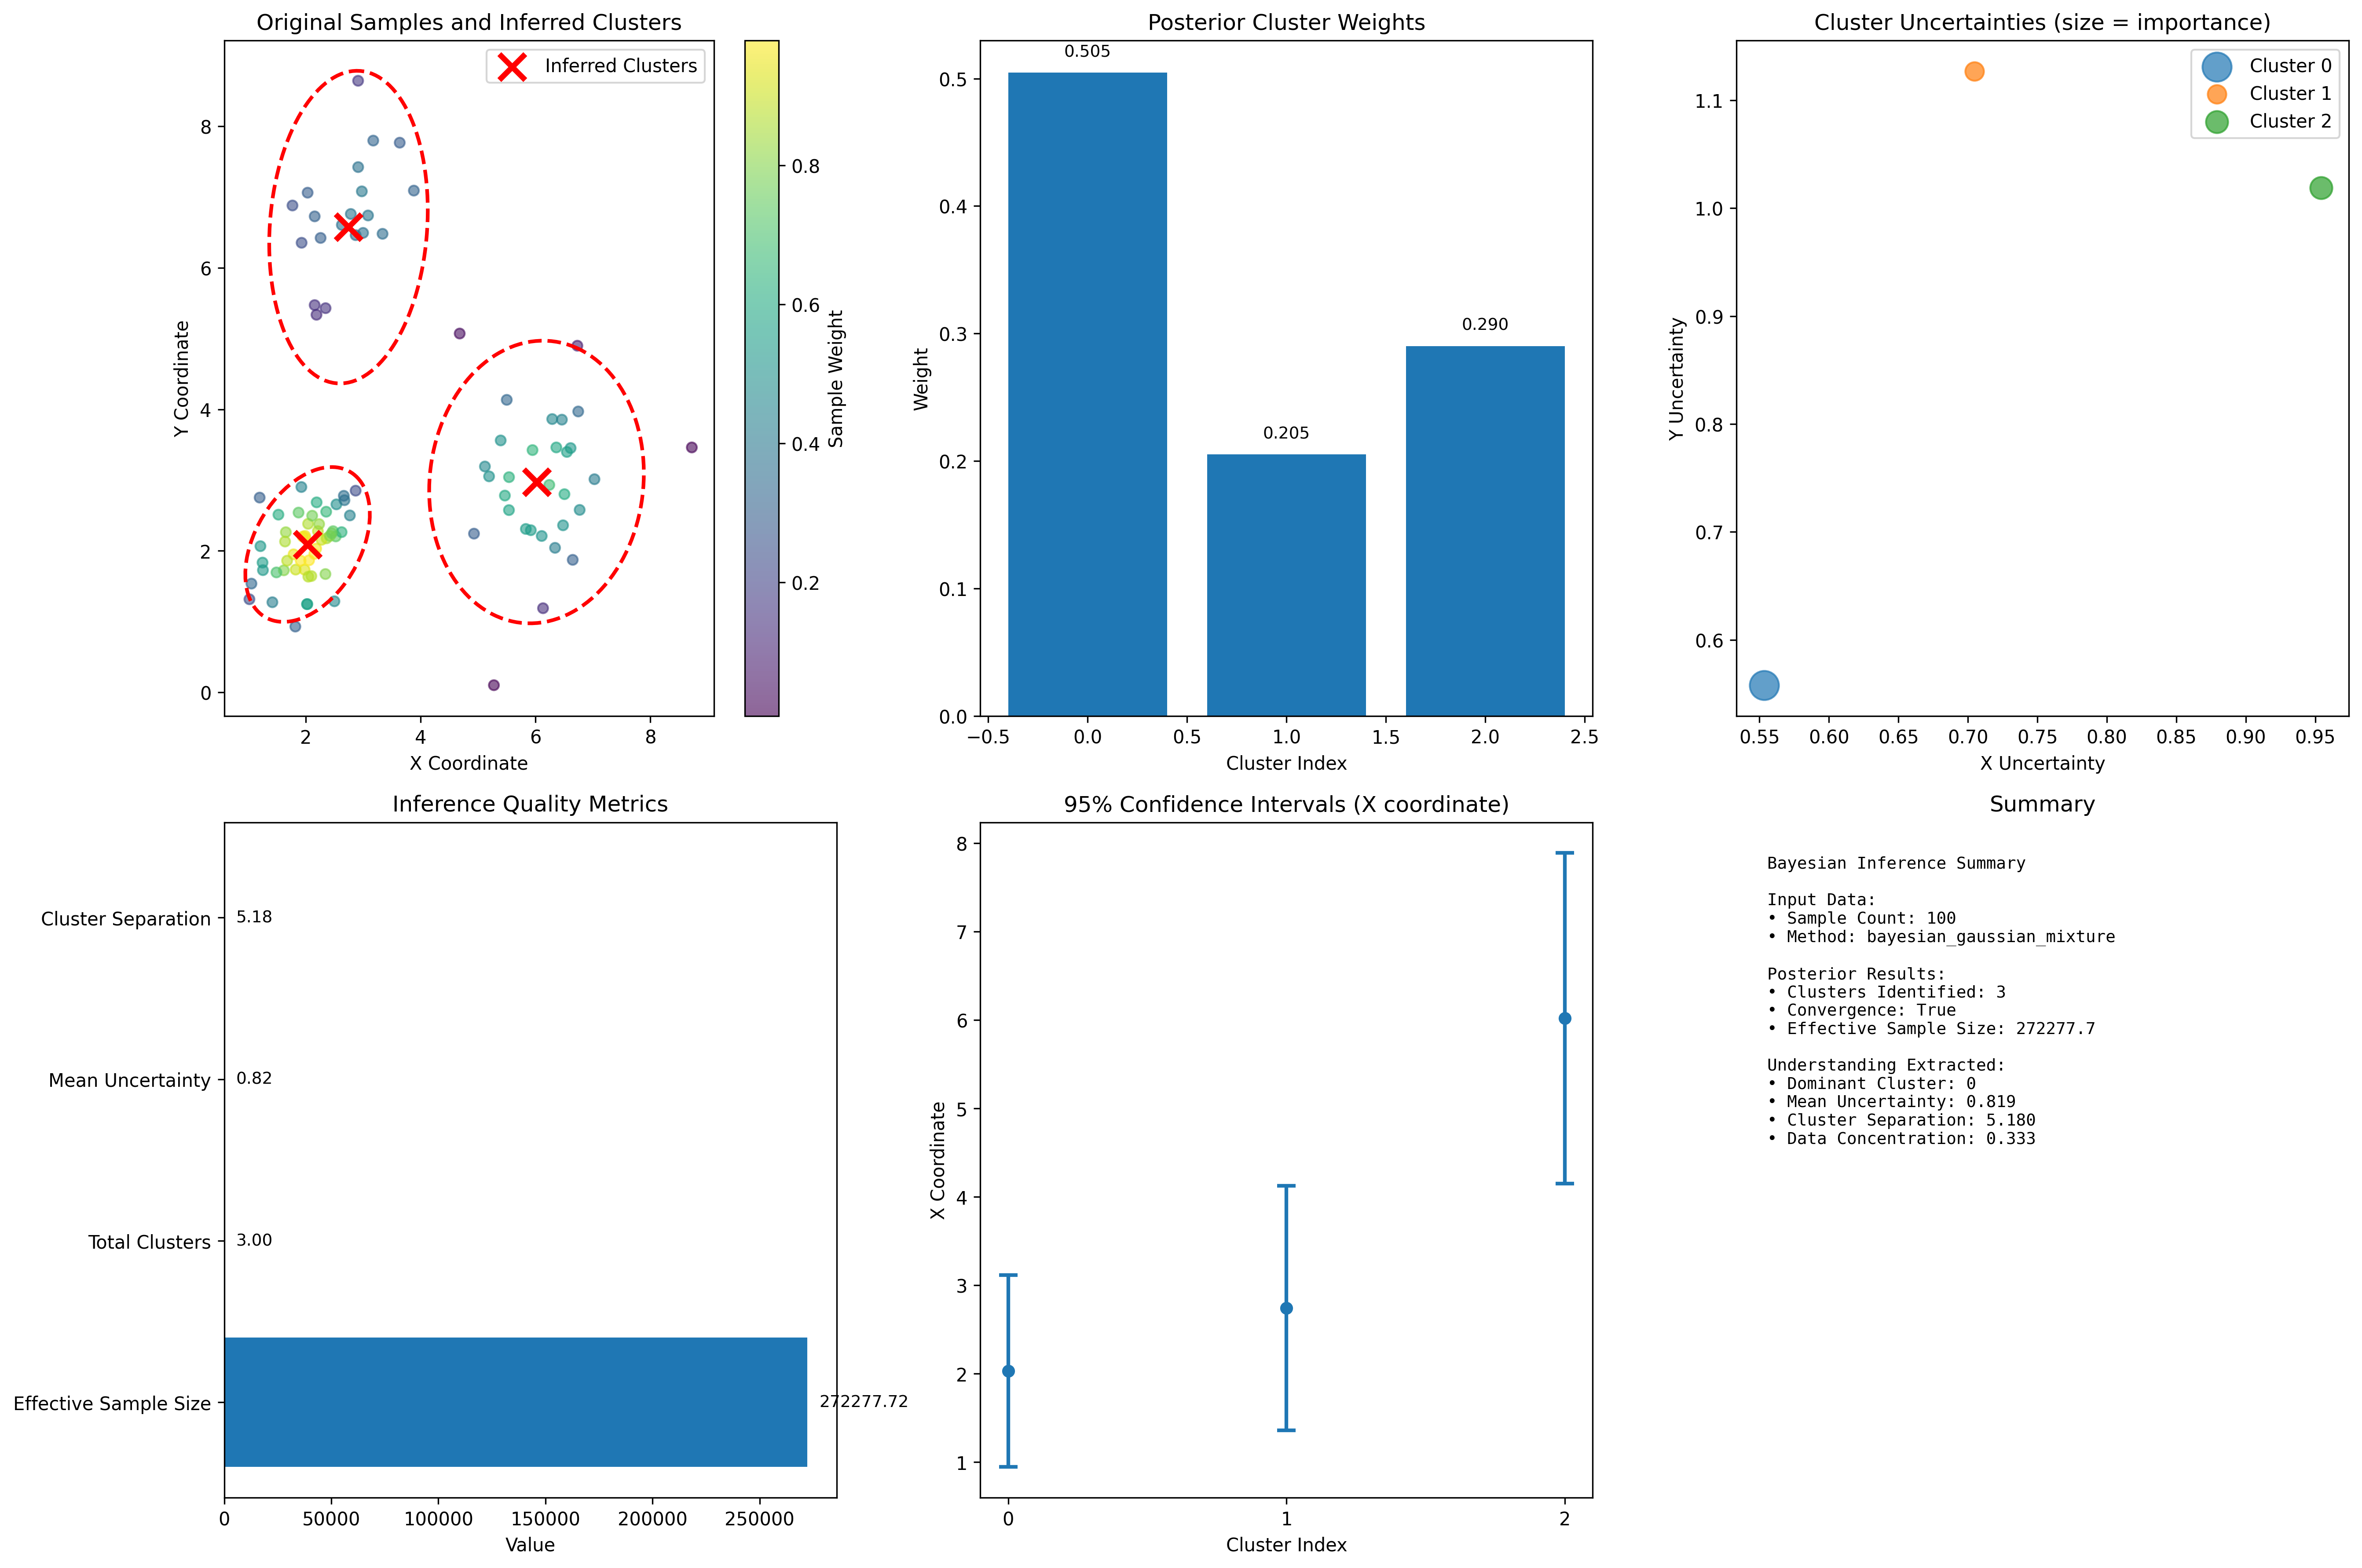
\includegraphics[width=\textwidth]{images/bayesian_inference_demo.png}
\caption{\textbf{Bayesian Inference on Constrained Stochastic Samples.} Comprehensive visualization of variational Bayesian analysis showing: (top left) original weighted samples overlaid with inferred cluster centers and 95\% confidence ellipses, (top center) posterior mixture weights indicating cluster importance, (top right) cluster uncertainty quantification with importance-weighted scatter plot, (bottom left) inference quality metrics including effective sample size and convergence diagnostics, (bottom center) 95\% credible intervals for cluster parameters, and (bottom right) complete inference summary statistics. The analysis successfully extracts semantic clusters from constraint-weighted samples with formal uncertainty quantification.}
\label{fig:bayesian-inference}
\end{figure}
